\part{Entrega 1}
\sloppy

\begin{center}
    \href{https://github.com/LukasWolff2002/PROYECTO_1_MCOC_ENTREGA_1}{Ver repositorio GitHub.}
\end{center}

\setcounter{section}{0}

\section{Introducción}

Actualmente existen diversos programas para realizar simulaciones de fluidos, lo cual facilita muchos procesos ingenieriles. La matemática que hay detrás de todos estos softwares no es simple y es prácticamente imposible realizar estos cálculos a mano. Ahora bien, es importante poder entender y analizar qué es lo que está ocurriendo detrás del análisis computacional, ya que de esta manera se pueden optimizar muchos procesos, mejorar el software o, mejor aún, no tener que comprar una licencia y escribir el código por cuenta propia.

En esta sección se buscará crear un código que simule el comportamiento del flujo en una ataguía utilizando diferencias finitas con el método de Laplace. Para lograr esto, se debe entender la ley de Darcy, la ecuación de continuidad y las diferencias finitas, ya que estos conceptos son fundamentales para desarrollar el código. Finalmente, se comprobará la eficacia del código comparando los resultados de caudal obtenidos en la parte anterior, además de una solución de ejemplo del problema 14.3 del libro \textbf{\cite{budhuSoilMechanics}}.

\section{Marco Teórico}

\subsection{Ley de Darcy}

La ley de Darcy expone lo siguiente:

\begin{equation}
    q = k \cdot i \cdot A
\end{equation}

Lo cual es análogo a:

\begin{equation}
    v = k \cdot i
\end{equation}

Donde \(i\) es el gradiente hidráulico. Discretizándolo en el espacio, se obtiene lo siguiente:

\begin{equation}
    i = \frac{dh}{dl} = \frac{dh}{dx}; \frac{dh}{dy}; \frac{dh}{dz}
\end{equation}

Sea lo siguiente:

\begin{figure}[H]
    \centering
    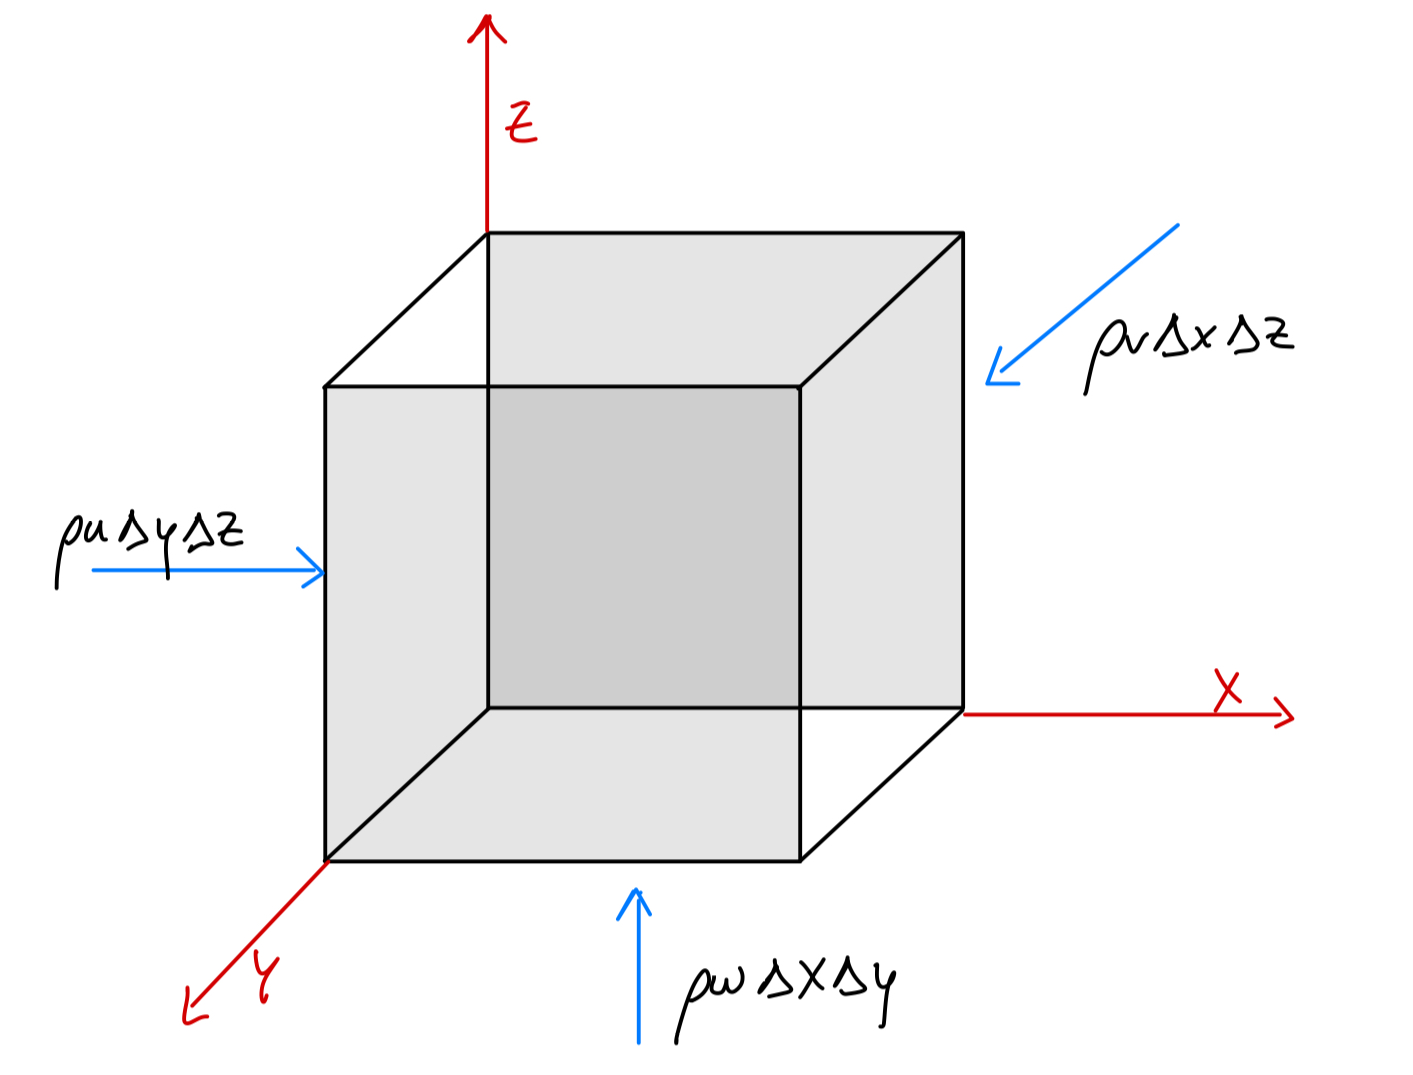
\includegraphics[width=0.5\textwidth]{FOTOS/in.jpg}
    \caption{Entrada al sistema}
    \label{fig:ley_darcy_in}
\end{figure}

La serie de Taylor expone que:

\begin{equation}
    f(x) = f(a) + \frac{df(a) \Delta X}{dx \cdot 1!} + ... + \frac{\Delta X^n}{n!} \cdot \frac{d^n f(a)}{dx^n}
\end{equation}

Por lo tanto, lo que sale del sistema es:

\begin{figure}[H]
    \centering
    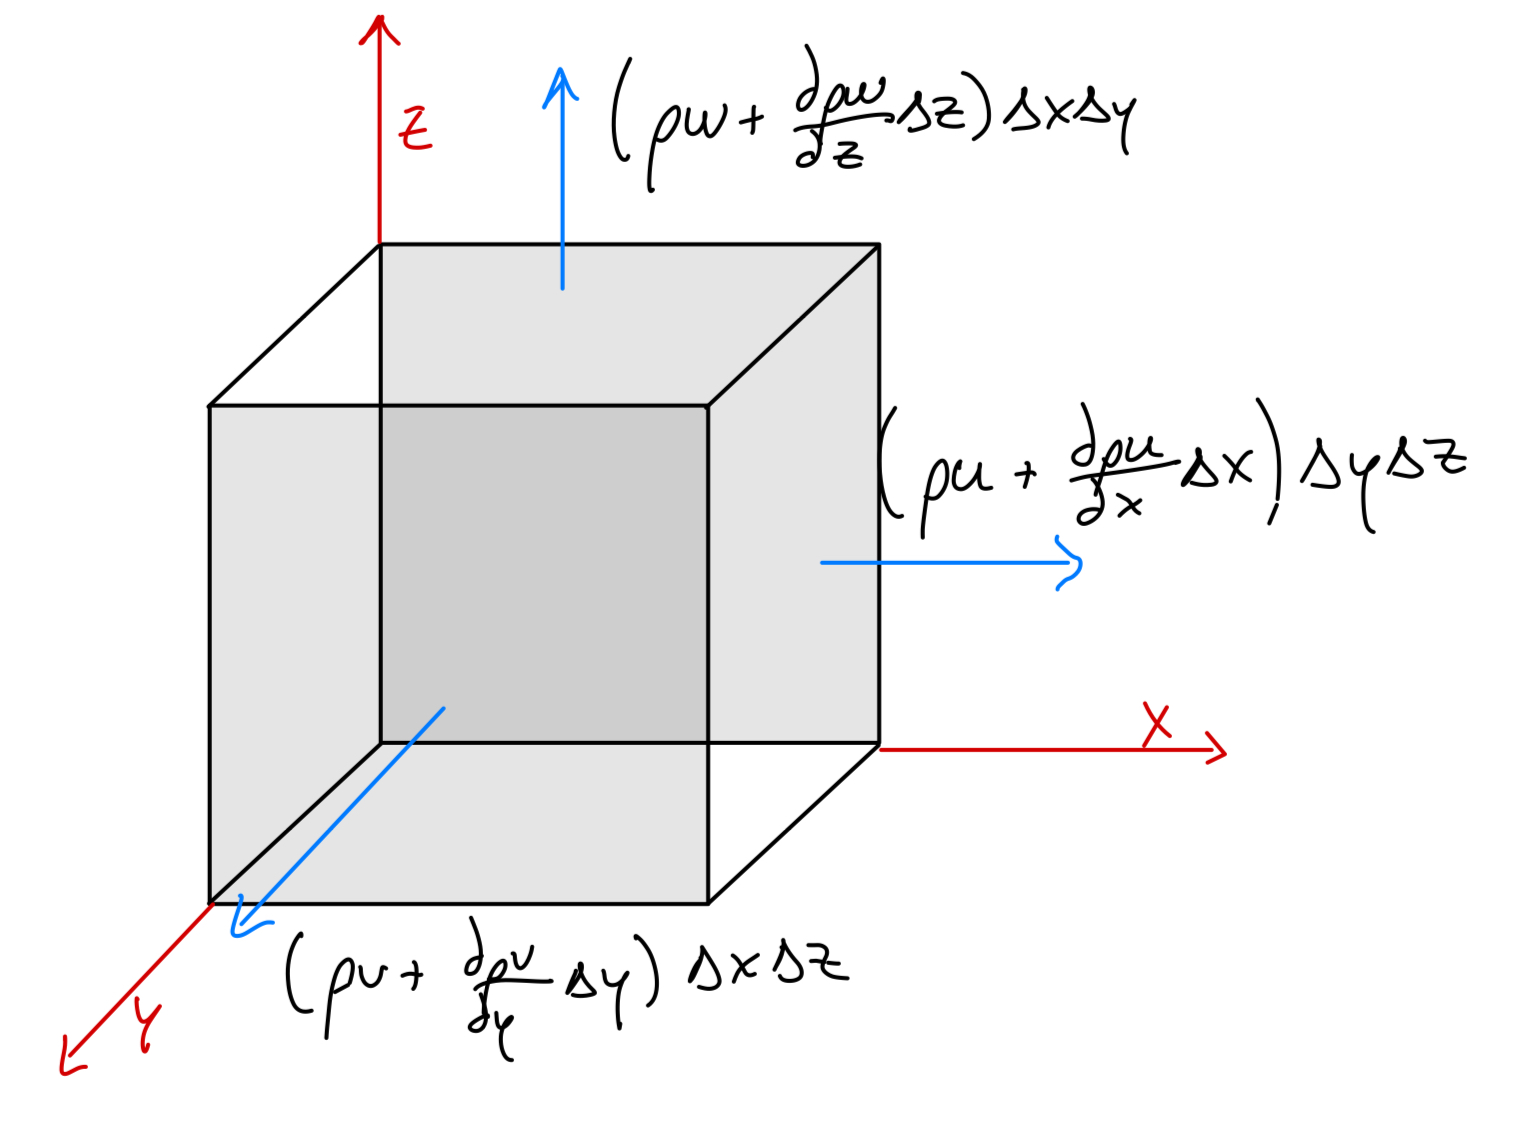
\includegraphics[width=0.5\textwidth]{FOTOS/out.jpg}
    \caption{Salida del sistema}
    \label{fig:ley_darcy_out}
\end{figure}

Luego, por conservación de masa:

\begin{equation}
    Q_{int} = Q_{out}
\end{equation}

De lo que se obtiene:

\begin{equation}
    \rho_u \Delta_y \Delta_z + \rho_v \Delta_x \Delta_z + \rho_w \Delta_x \Delta_y = (\rho_u + \frac{d\rho_u \Delta x}{dx})\Delta_y \Delta_z + (\rho_v + \frac{d\rho_v \Delta y}{dy})\Delta_x \Delta_z + (\rho_w + \frac{d\rho_w \Delta z}{dz})\Delta_x \Delta_y
\end{equation}

Simplificando:

\begin{equation}
    \Delta_x \Delta_y \Delta_z = Volumen
\end{equation}

Pero el fluido, al ser agua, es incompresible, por lo tanto:

\begin{equation}
   -\rho(\frac{du}{dx}+ \frac{dv}{dy}+ \frac{dw}{dz}) = 0
\end{equation}

Lo que es análogo a decir:

\begin{equation}
    -\rho \nabla \cdot \vec{v} = 0 = \nabla \cdot \vec{v}
\end{equation}

Por lo tanto, si reemplazamos en la ley de Darcy, obtenemos:

\begin{equation}
    V_x = k_x\cdot \frac{dh}{dx}; V_y = k_y\cdot \frac{dh}{dy}; V_z = k_z\cdot \frac{dh}{dz}
\end{equation}

Incorporando la ecuación de continuidad, se obtiene:

\begin{equation}
    \nabla \cdot \vec{V} = \nabla \cdot (k \cdot \vec{i}) = 0
\end{equation}

Asumiendo un análisis en 2D, se obtiene:

\begin{equation}
    \frac{d}{dx}(k_x \cdot \frac{dh}{dx}) + \frac{d}{dy}(k_y \cdot \frac{dh}{dy}) = 0
\end{equation}

Pero sabemos, o mejor dicho, suponemos que:

\begin{equation}
    k_x = k_y = k
\end{equation}

Por lo tanto:

\begin{equation}
    k \nabla^2 h = 0
\end{equation}

De esta forma, podemos representar el laplaciano con diferencias finitas.

\subsection{Diferencias Finitas}

\subsubsection{Diferencias Hacia Adelante}

\begin{equation}
    h(x + \Delta x) = h(x) + \frac{dh}{dx} \Delta x + ...
\end{equation}

\subsubsection{Diferencias Hacia Atrás}

\begin{equation}
    h(x - \Delta x) = h(x) - \frac{dh}{dx} \Delta x + ...-...+
\end{equation}

\subsubsection{Diferencias Centrales}

Se representa como la suma de una diferencia hacia adelante y hacia atrás, obteniendo:

\begin{equation}
    h(x + \Delta x) + h(x - \Delta x) = h(x) + \frac{d^2h}{dx^2}\frac{\Delta x}{2!} + ...(los pares)
\end{equation}

Donde la incógnita que se busca es $\frac{d^2h}{dx^2}$, por lo tanto, despejando, se obtiene:

\begin{equation}
    \frac{d^2h}{dx^2} = \frac{h(x + \Delta x) - 2h(x) + h(x - \Delta x)}{\Delta x^2}
\end{equation}

\begin{equation}
    \frac{dh}{dx} = \frac{h(x + \Delta x) - h(x)}{\Delta x}
\end{equation}

Lo cual se puede llevar a una grilla:

\begin{figure}[H]
    \centering
    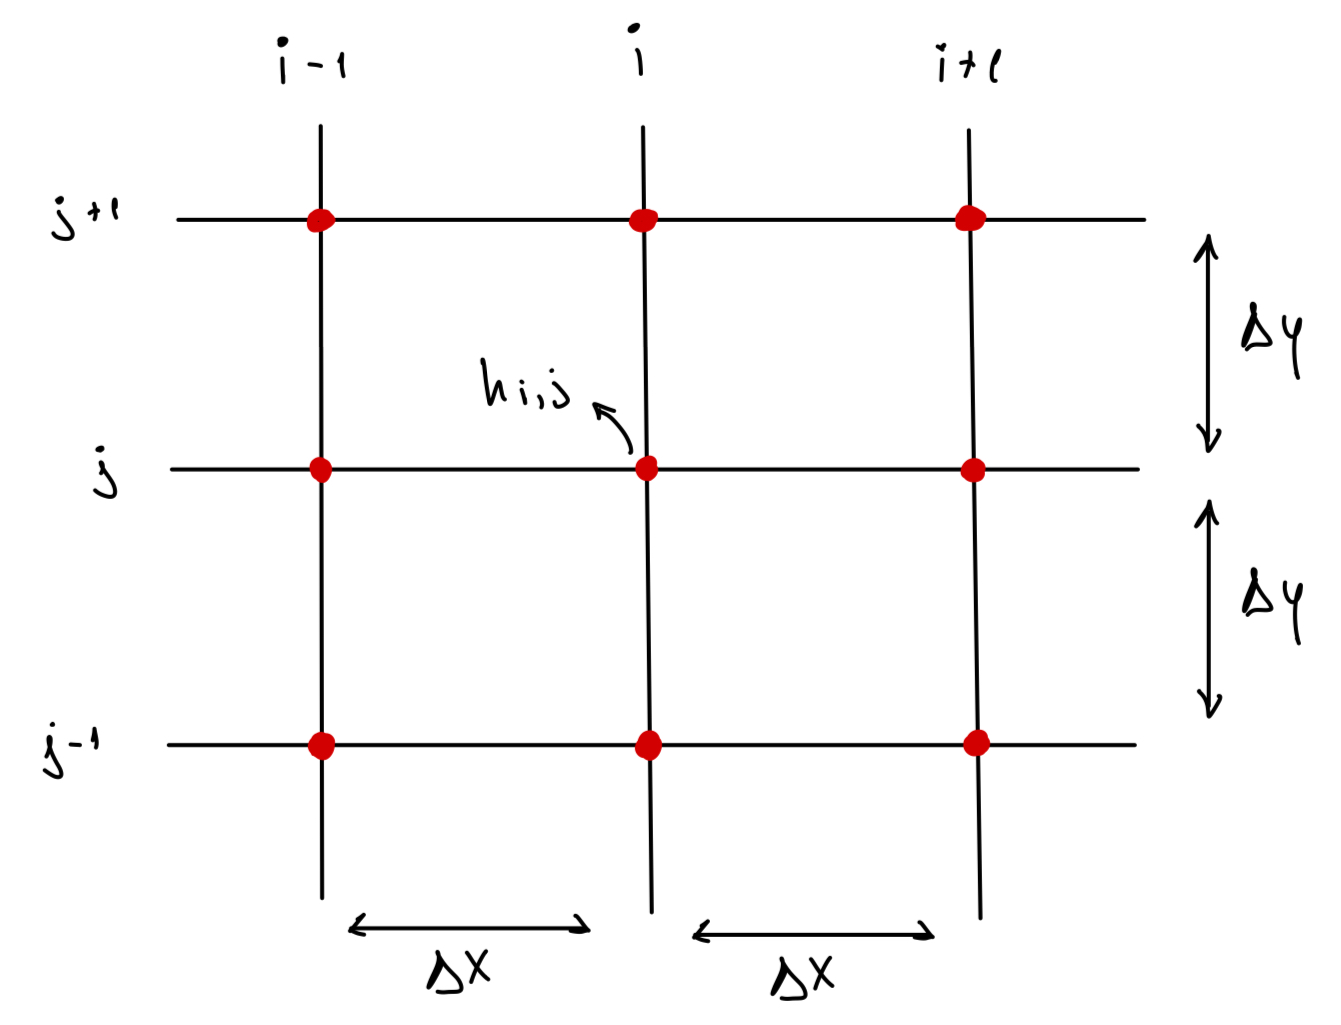
\includegraphics[width=0.5\textwidth]{FOTOS/grilla.jpg}
    \caption{Grilla}
\end{figure}

Donde se puede representar la ecuación de Laplace como:

\begin{equation}
    \frac{d^2h}{dx^2} = \frac{h_{i+1,j} + h_{i-1,j} - 2h_{i,j}}{\Delta x^2}
\end{equation}

\begin{equation}
    \frac{dh}{dx} = \frac{h_{+1,j} + h_{i+1,j}}{2\Delta x}
\end{equation}

Por lo tanto, podemos expresar la ley de Darcy con diferencias centrales, obteniendo:

\begin{equation}
    \frac{k}{\Delta^2}(h_{i+1,j} + h_{i-1,j} + h_{i,j+1} + h_{i,j-1} - 4h_{i,j}) = 0
\end{equation}

Donde se busca:

\begin{equation}
    h_{i,j} = \frac{1}{4}(h_{i+1,j} + h_{i-1,j} + h_{i,j+1} + h_{i,j-1})
\end{equation}

De esta forma, es posible obtener las diferentes variaciones en el potencial, a partir de los datos conocidos en la grilla (condiciones de borde).

\newpage
\section{Desarrollo}

Para explicar el desarrollo del código, se utilizará el Caso Ejemplo 1, empleando una grilla de 10x10. En primer lugar, se desarrolla la matriz de potencial con las condiciones de borde:

\begin{center}
    \begin{tabular}{|c|c|c|c|c|c|c|c|c|c|} 
        \hline
        \textbf{0} & \textbf{300} & \textbf{300} & \textbf{300} & \textbf{300} & \textbf{0} & \textbf{380} & \textbf{380} & \textbf{380} & \textbf{0} \\
        \hline
        \textbf{0} & \textbf{300} & \textbf{300} & \textbf{300} & \textbf{300} & \textbf{0} & 1 & 1 & 1 & \textbf{0} \\
        \hline
        \textbf{0} & \textbf{300} & \textbf{300} & \textbf{300} & \textbf{300} & \textbf{0} & 1 & 1 & 1 & \textbf{0} \\
        \hline
        \textbf{0} & \textbf{300} & \textbf{300} & \textbf{300} & \textbf{300} & \textbf{0} & 1 & 1 & 1 & \textbf{0} \\
        \hline
        \textbf{0} & 1 & 1 & 1 & 1 & 1 & 1 & 1 & 1 & \textbf{0} \\
        \hline
        \textbf{0} & 1 & 1 & 1 & 1 & 1 & 1 & 1 & 1 & \textbf{0} \\
        \hline
        \textbf{0} & 1 & 1 & 1 & 1 & 1 & 1 & 1 & 1 & \textbf{0} \\
        \hline
        \textbf{0} & 1 & 1 & 1 & 1 & 1 & 1 & 1 & 1 & \textbf{0} \\
        \hline
        \textbf{0} & 1 & 1 & 1 & 1 & 1 & 1 & 1 & 1 & \textbf{0} \\
        \hline
        \textbf{0} & \textbf{0} & \textbf{0} & \textbf{0} & \textbf{0} & \textbf{0} & \textbf{0} & \textbf{0} & \textbf{0} & \textbf{0} \\
        \hline
    \end{tabular}
\end{center}

Donde se observan las condiciones de impermeabilidad representadas por \textbf{(0)}, la condición de inicio de flujo \textbf{(380)} y la condición de flujo final \textbf{(300)}. Por razones de lógica de código, se utiliza este valor en los espacios con aire. Luego, iterando según la teoría expuesta anteriormente y manteniendo las condiciones de borde, se obtiene lo siguiente:

\begin{center}
    \begin{tabular}{|c|c|c|c|c|c|c|c|c|c|} 
        \hline
        \textbf{0} & \textbf{300} & \textbf{300} & \textbf{300} & \textbf{300} & \textbf{0} & \textbf{380} & \textbf{380} & \textbf{380} & \textbf{0} \\
        \hline
        \textbf{0} & \textbf{300} & \textbf{300} & \textbf{300} & \textbf{300} & \textbf{0} & 365 & 366 & 367 & \textbf{0} \\
        \hline
        \textbf{0} & \textbf{300} & \textbf{300} & \textbf{300} & \textbf{300} & \textbf{0} & 351 & 353 & 354 & \textbf{0} \\
        \hline
        \textbf{0} & \textbf{300} & \textbf{300} & \textbf{300} & \textbf{300} & 317 & 334 & 341 & 343 & \textbf{0} \\
        \hline
        \textbf{0} & 303 & 304 & 305 & 309 & 317 & 327 & 332 & 335 & \textbf{0} \\
        \hline
        \textbf{0} & 306 & 307 & 309 & 312 & 318 & 323 & 327 & 329 & \textbf{0} \\
        \hline
        \textbf{0} & 309 & 310 & 311 & 314 & 318 & 321 & 324 & 326 & \textbf{0} \\
        \hline
        \textbf{0} & 310 & 311 & 313 & 315 & 318 & 320 & 322 & 324 & \textbf{0} \\
        \hline
        \textbf{0} & 311 & 312 & 313 & 315 & 318 & 320 & 322 & 323 & \textbf{0} \\
        \hline
        \textbf{0} & \textbf{0} & \textbf{0} & \textbf{0} & \textbf{0} & \textbf{0} & \textbf{0} & \textbf{0} & \textbf{0} & \textbf{0} \\
        \hline
    \end{tabular}         
\end{center}

Este es un proceso iterativo, donde se determina que la condición de finalización corresponde a un error de \textbf{1e-6}.
\\ \\
Posteriormente, es posible obtener las matrices de velocidades de la siguiente manera:

\begin{lstlisting}[language=Python]
    # Calcular el gradiente del potencial (flujo de velocidad)
    dy, dx = np.gradient(potential, dy, dx)

    # Luego, el gradiente se multiplica por la permeabilidad K
    velocity_x = -dx * K 
    velocity_y = -dy * K
\end{lstlisting}

A continuación, se presentan los distintos resultados obtenidos, donde se utilizó una grilla de 40x40 en cada caso.

\subsection{Caso 1}

\begin{figure}[H]
    \centering
    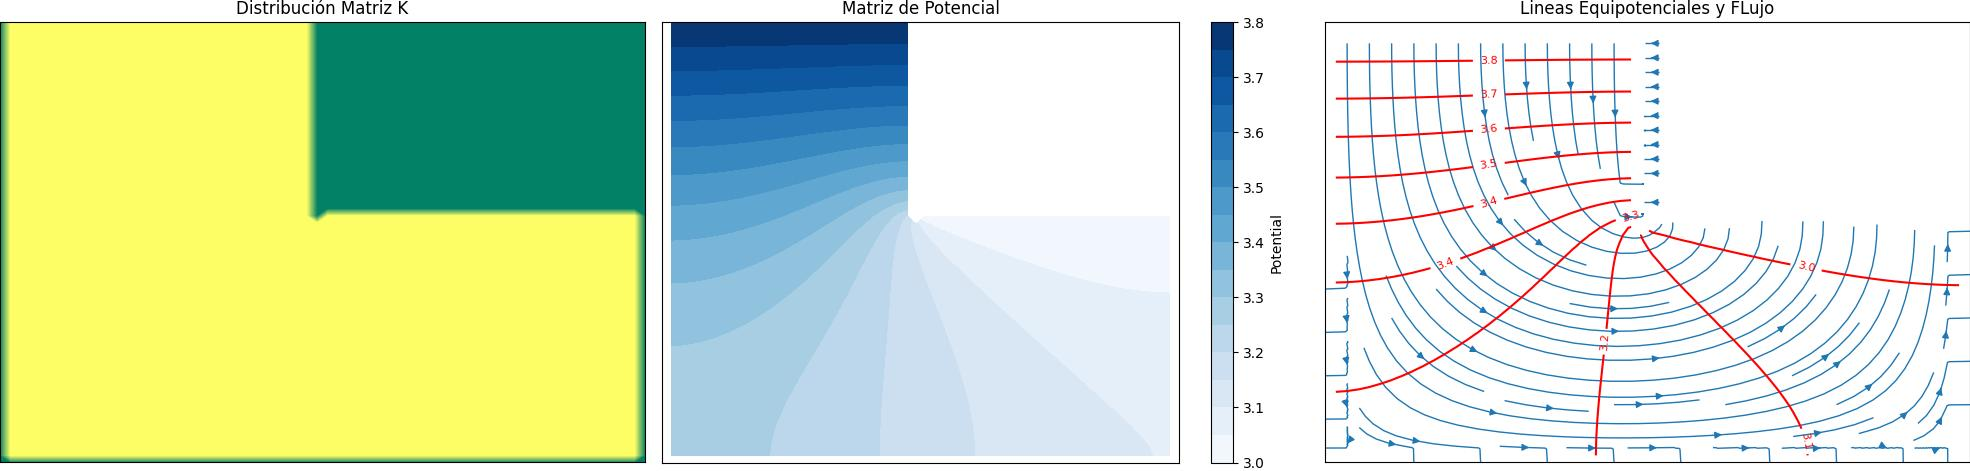
\includegraphics[width=1\textwidth]{GRAFICOS/laplace_caso_1.jpg}
    \caption{Caso 1}
    \label{fig:caso_1}
\end{figure}

Se alcanzó la convergencia en la \textbf{iteración 13775}.

\subsection{Caso 2}

\begin{figure}[H]
    \centering
    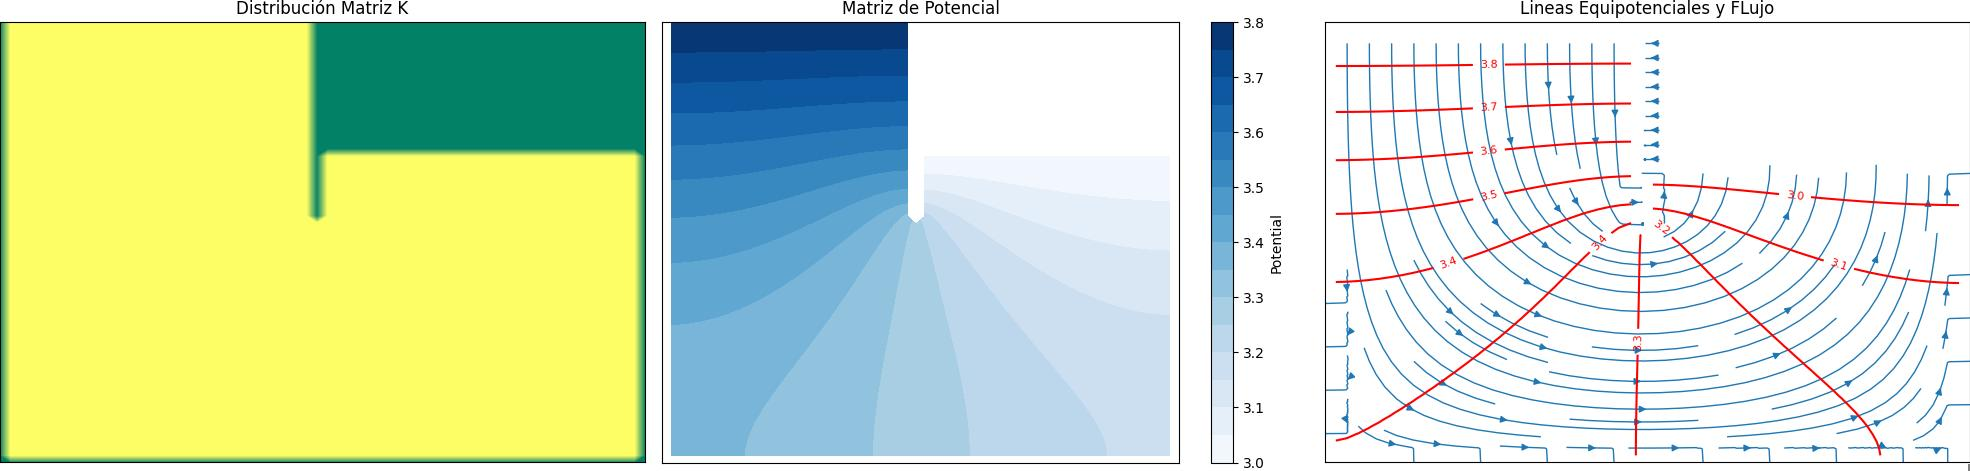
\includegraphics[width=1\textwidth]{GRAFICOS/laplace_caso_2.jpg}
    \caption{Caso 2}
    \label{fig:caso_2}
\end{figure}

Se alcanzó la convergencia en la \textbf{iteración 19556}.

\subsection{Caso 3}

\begin{figure}[H]
    \centering
    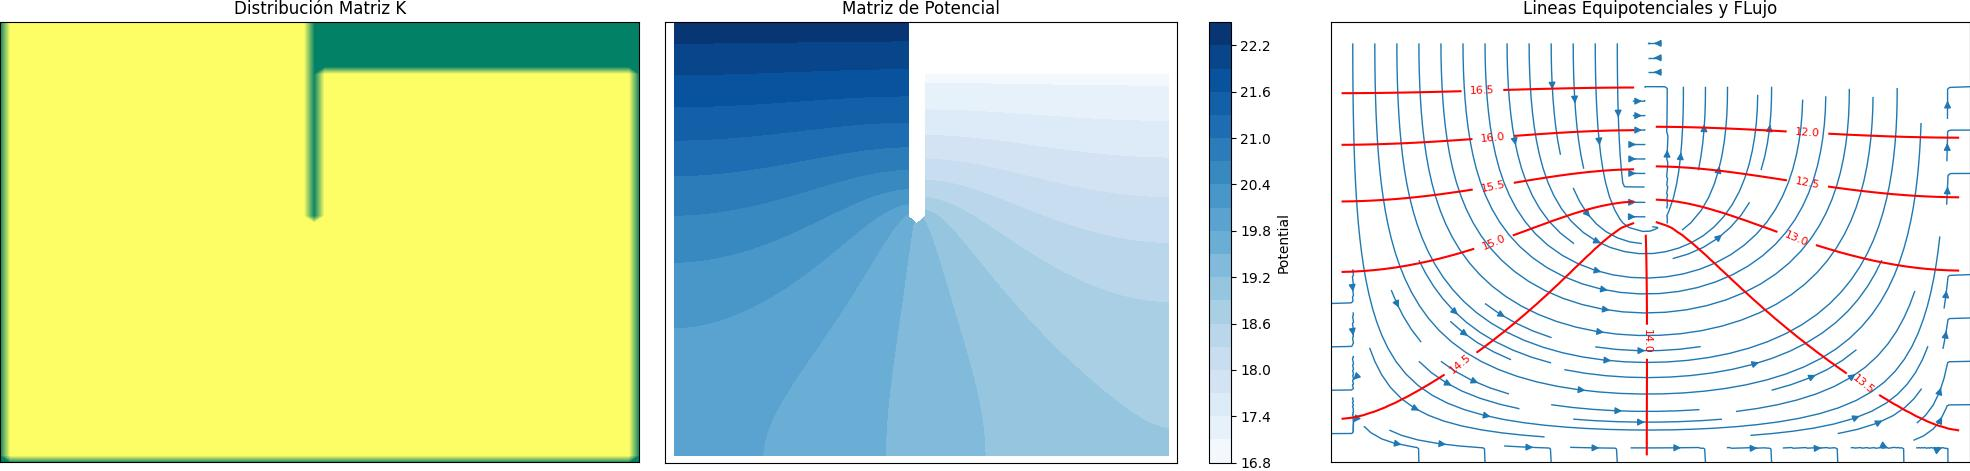
\includegraphics[width=1\textwidth]{GRAFICOS/laplace_caso_3.jpg}
    \caption{Caso 3}
    \label{fig:caso_3}
\end{figure}

Se alcanzó la convergencia en la \textbf{iteración 26253}.

\subsection{Caso Ejemplo Libro}

\begin{figure}[H]
    \centering
    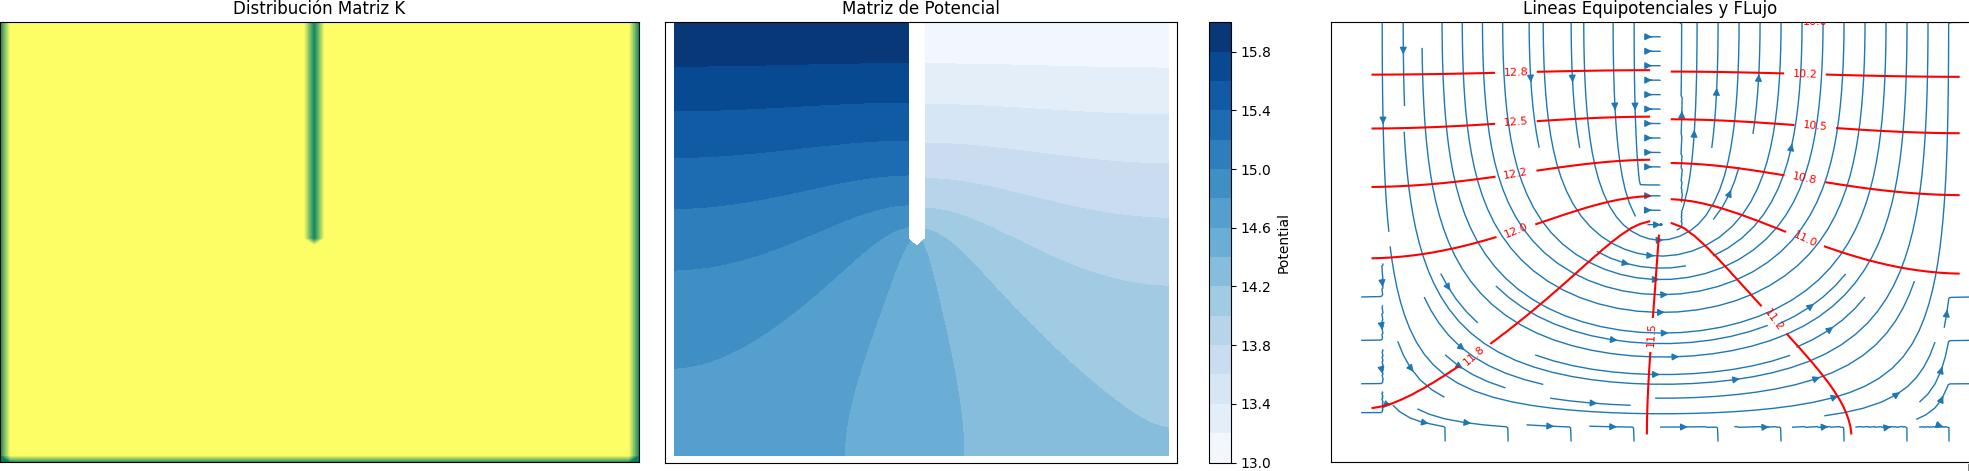
\includegraphics[width=1\textwidth]{GRAFICOS/laplace_caso_ejemplo.jpg}
    \caption{Caso Ejemplo Libro}
    \label{fig:caso_ejemplo}
\end{figure}

Se alcanzó la convergencia en la \textbf{iteración 28172}.
\\ \\
La velocidad de salida obtenida fue de \textbf{3.24e-06} m/s, de esta manera se corrobora que el código está correctamente calibrado, ya que el resultado expuesto por el libro es de \textbf{3.2e-06} m/s.
\\ \\
Además, se realizó un caso doble para observar cómo afecta la condición de impermeabilidad de la barrera derecha en el flujo:

\begin{figure}[H]
    \centering
    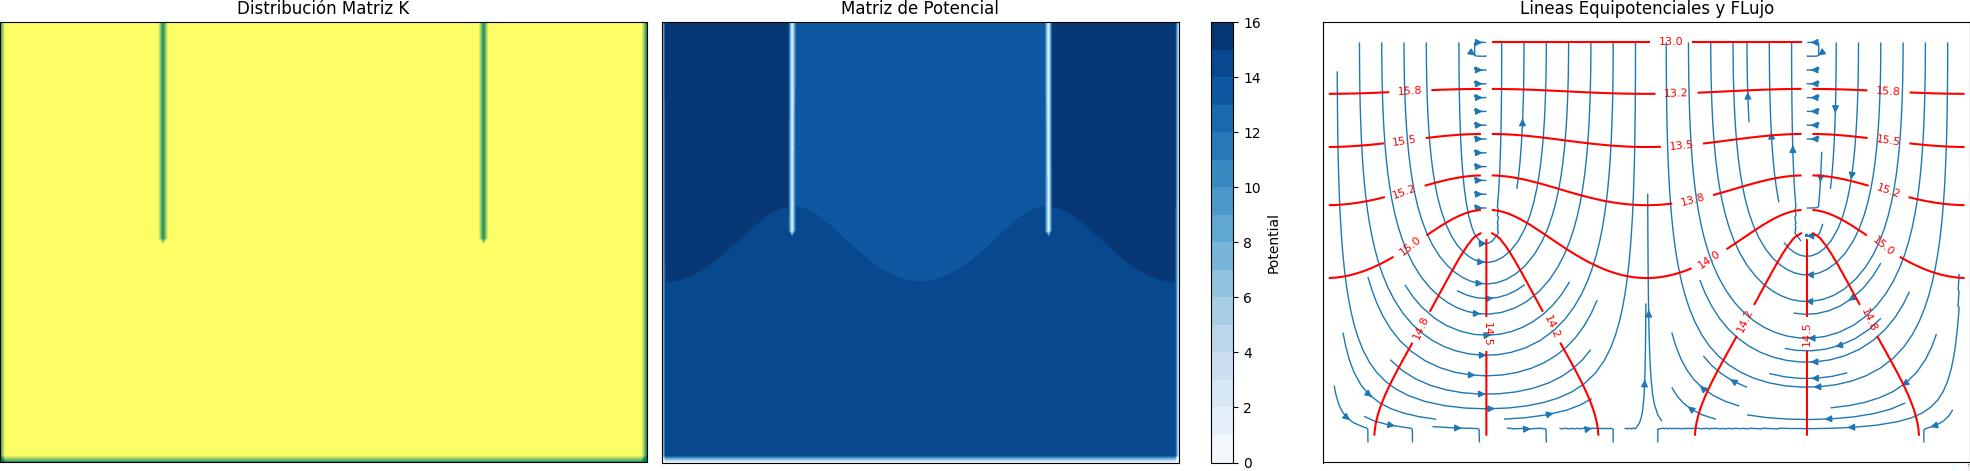
\includegraphics[width=1\textwidth]{GRAFICOS/laplace_caso_ejemplo_doble.jpg}
    \caption{Caso Ejemplo Libro Doble}
    \label{fig:caso_ejemplo_doble}
\end{figure}

Se alcanzó la convergencia en la \textbf{iteración 16708}.
\\ \\
La velocidad de salida obtenida fue de \textbf{2.63e-06} m/s.

\subsection{Caudales Según Modelo Entrega 0}

Considerando los caudales obtenidos en la entrega 0 (\ref{fig:Q_inf}), y teniendo en cuenta que cada cuadrícula representa un metro y, además, hay una profundidad \(Z\) de un metro, es posible calcular el caudal puntual:

\begin{table}[H]
    \centering
    \begin{tabular}{|c|c|c|c|}
      \hline
      \textbf{Caso} & \textbf{Caudal de Infiltración [$m/día$]} & \textbf{Caudal Según Laplace [$m/día$]} & \textbf{Error [\%]} \\ \hline
      1 & 0.97 & 1.21  &  24.7  \\ \hline
      2 & 0.72 &  0.99 &  36.0 \\ \hline
      3 & 0.57 &  0.66 &  15.8  \\
      \hline
    \end{tabular}
    \caption{Caudal de Infiltración}
    \label{fig:Q_inf}
\end{table}

\section{Análisis}

Se puede observar que la teoría expuesta en la entrega 0 fue corroborada correctamente. El error observado es muy bajo, lo cual se atribuye a una impermeabilidad no perfecta, lo que se asemeja más a la realidad.
\\ \\
Además, se observa que los gráficos de potencial tienen una lógica correcta, donde se pueden identificar adecuadamente las líneas equipotenciales. Comparando con la entrega 0, se puede concluir que los gráficos realizados mediante Python están correctamente hechos. Sin embargo, faltó conectar las líneas equipotenciales a los bordes izquierdo y derecho.
\\ \\
Finalmente, se observa que en el caso doble, el caudal disminuye, lo cual tiene sentido, ya que se está eliminando una condición de impermeabilidad. Además, se puede observar que la interacción entre ambos flujos al momento de colisionar ocurre de manera correcta.

\section{Conclusión}

En conclusión, todos los objetivos propuestos en esta entrega fueron logrados de manera satisfactoria. En particular, se logró generar un modelo computacional capaz de recrear el flujo en una ataguía mediante diferencias finitas.
\\ \\
Posteriormente, este modelo fue calibrado mediante una comparación con los caudales teóricos, donde el error observado está dentro de un rango esperado y considerado aceptable.
\\ \\
Finalmente, se desarrolló un código para observar el comportamiento de dos flujos que colisionan, donde se observó que el caudal disminuye al eliminar una condición de impermeabilidad, lo cual es un resultado esperado.
\\ \\
Considerando todo lo anteriormente expuesto, se puede concluir que la presente entrega fue exitosa.
